All three schemes (\cref{scheme A,scheme B,scheme C}) were implemented with $\lambda = [0.5,0.8,1,2]$, and the solutions at $t=2$ are reported for $f_1$ in \cref{f1 figures} and $f_2$ in \cref{f2 figures}.

For all cases, the solutions matched well with the theory derived above. 
That is, all schemes were proven to be stable.
Although the error\footnote{The discrete L2 norm was reported on each subfigure for reference, calculated using the Trapezoid Rule.} grew quite large for $\lambda =2$ in \textit{all} cases, the solutions did \textit{not} go to $\pm \infty$ in finite time.
In this case, we deduce that not all $\lambda$ values are applicable to solving a PDE.

Generally, the error reduced for each scheme as $\lambda \rightarrow 1$, aside from \cref{weird leap frog}, indicating a convergence of error as $k\rightarrow h$.
However, the error grows rapidly once $k>h$.
\Cref{weird leap frog} can be explained by the results in~\cref{sec:q3}, where the scheme may become unstable when $\lambda \geq 1$ (this point can be thought of as a bifurcation in stability analysis), which is supported by the many orders of magnitude difference between Scheme \textbf{C} and Schemes \textbf{A} and \textbf{B} once $\lambda =2$.
Overall, it appears clear that Forward-Time-Backward-Space (FTBS) and Leap-Frog were the best methods in terms of accuracy and convergence to their respective best numerical answer.
However, it appears that FTBS performed better overall, as it avoided much of the ``wobbling'' observed by the Leap-Frog scheme.
That said, Leap-Frog appears much better suited for solving continuous, smooth schemes, even at lower $\lambda$ values, implying that a less-fine spatial discretization could be used, which would speed up the computation.
\\ \\
\noindent \textit{Note:} Because Scheme \textbf{C} depends on the previous \textit{two} time steps, the first time step taken after the initial conditions is found using Scheme \textbf{A}.
Additionally, the code was created such that the periodic boundary condition was satisfied for $f_1$ by demanding $x-t\in [-1,1]$.
This was achieved by creating a \texttt{while} loop which shifts the input by the length of the interval (in this case, by adding 2).
Python code is available upon request by contacting \url{lipohlmann@unm.edu}.

\begin{figure}
    \centering
    \begin{subfigure}{0.3\linewidth}
        \centering
        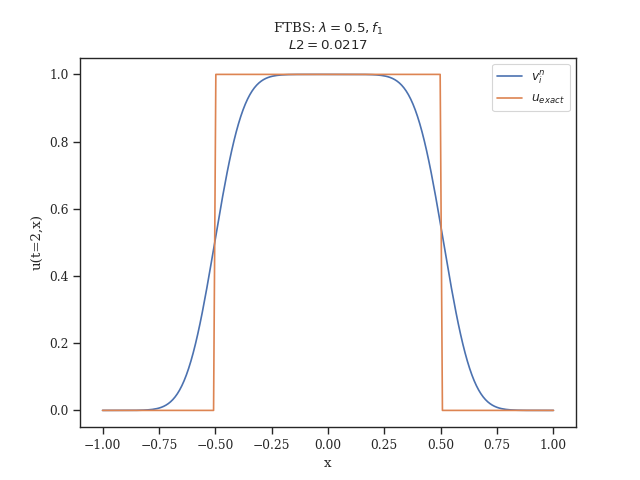
\includegraphics[width=\linewidth]{figures/FTBS/FTBS_lambda=0.5,f1}
        \caption{FTBS, $\lambda = 0.5$}
    \end{subfigure}
    \hfill
    \begin{subfigure}{0.3\linewidth}
        \centering
        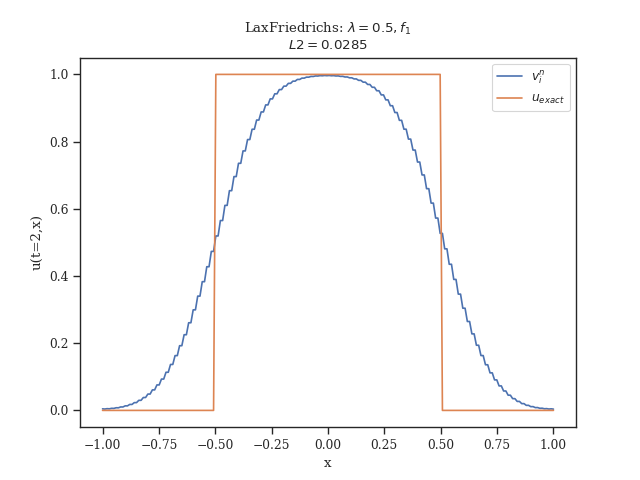
\includegraphics[width=\linewidth]{figures/LaxFriedrichs/LaxFriedrichs_lambda=0.5,f1}
        \caption{Lax-Friedrichs, $\lambda =0.5$}
    \end{subfigure}
    \hfill
    \begin{subfigure}{0.3\linewidth}
        \centering
        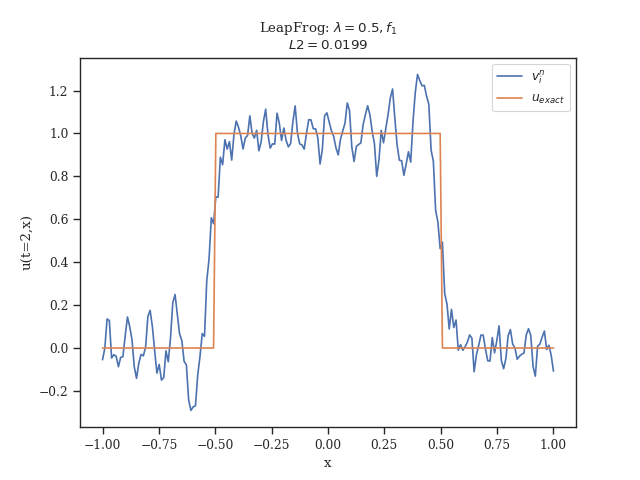
\includegraphics[width=\linewidth]{figures/LeapFrog/LeapFrog_lambda=0.5,f1}
        \caption{Leap-Frog, $\lambda =0.5$}
    \end{subfigure}
    \hfill
    \vspace{1cm}
    \begin{subfigure}{0.3\linewidth}
        \centering
        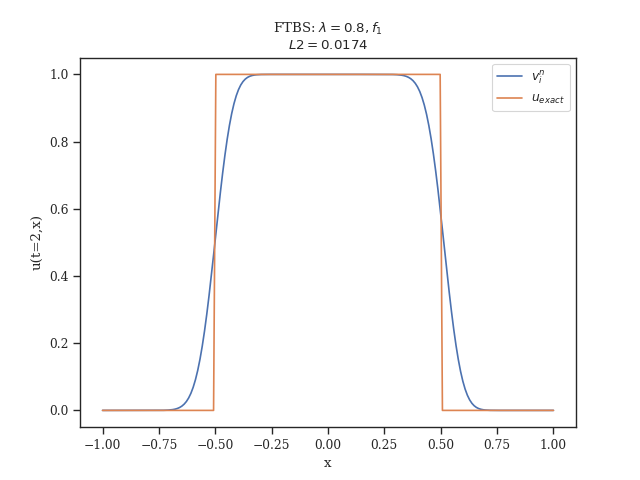
\includegraphics[width=\linewidth]{figures/FTBS/FTBS_lambda=0.8,f1}
        \caption{FTBS, $\lambda = 0.8$}
    \end{subfigure}
    \hfill
    \begin{subfigure}{0.3\linewidth}
        \centering
        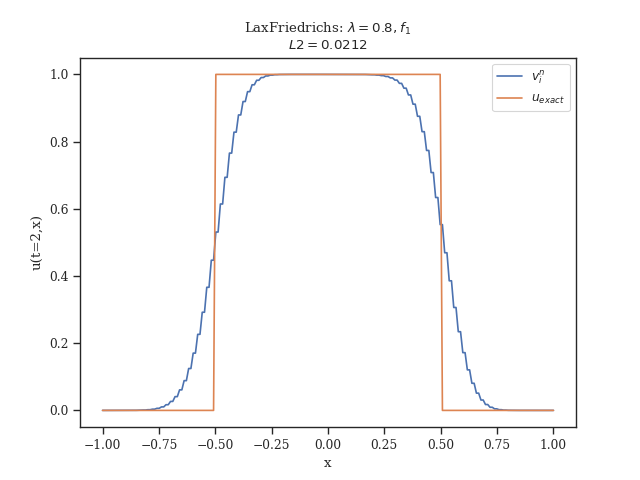
\includegraphics[width=\linewidth]{figures/LaxFriedrichs/LaxFriedrichs_lambda=0.8,f1}
        \caption{Lax-Friedrichs, $\lambda =0.8$}
    \end{subfigure}
    \hfill
    \begin{subfigure}{0.3\linewidth}
        \centering
        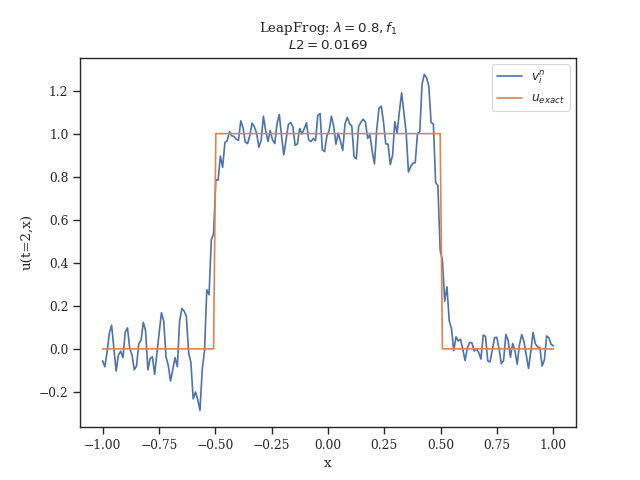
\includegraphics[width=\linewidth]{figures/LeapFrog/LeapFrog_lambda=0.8,f1}
        \caption{Leap-Frog, $\lambda =0.8$}
    \end{subfigure}
    \hfill
    \vspace{1cm}
    \begin{subfigure}{0.3\linewidth}
        \centering
        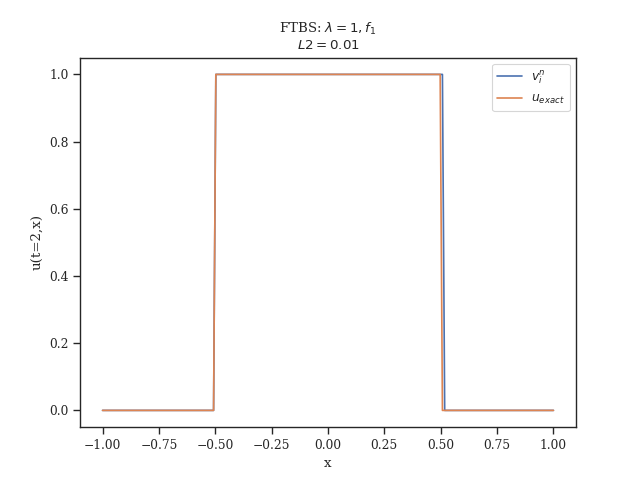
\includegraphics[width=\linewidth]{figures/FTBS/FTBS_lambda=1,f1}
        \caption{FTBS, $\lambda = 1$}
    \end{subfigure}
    \hfill
    \begin{subfigure}{0.3\linewidth}
        \centering
        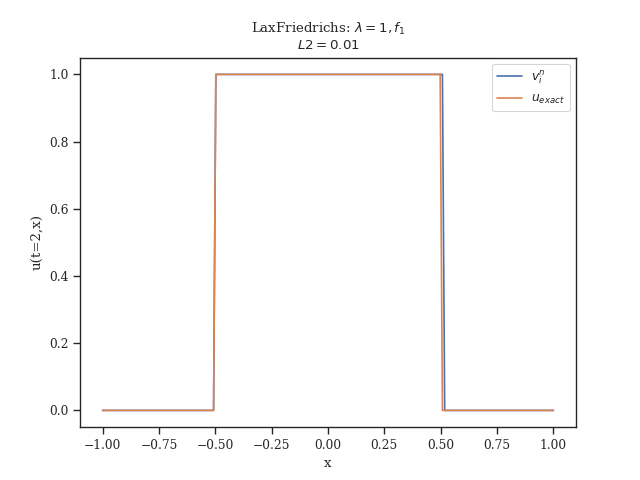
\includegraphics[width=\linewidth]{figures/LaxFriedrichs/LaxFriedrichs_lambda=1,f1}
        \caption{Lax-Friedrichs, $\lambda =1$}
    \end{subfigure}
    \hfill
    \begin{subfigure}{0.3\linewidth}
        \centering
        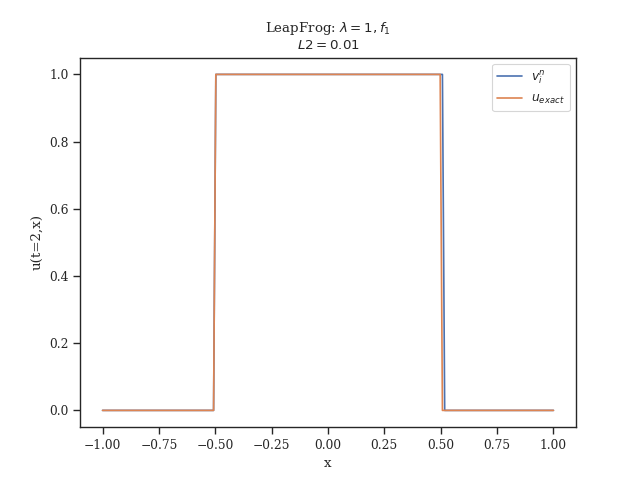
\includegraphics[width=\linewidth]{figures/LeapFrog/LeapFrog_lambda=1,f1}
        \caption{Leap-Frog, $\lambda =1$}
    \end{subfigure}
    \hfill
    \vspace{1cm}
    \begin{subfigure}{0.3\linewidth}
        \centering
        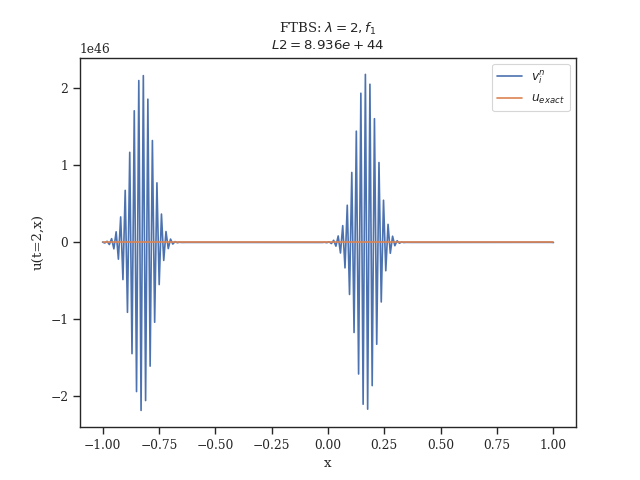
\includegraphics[width=\linewidth]{figures/FTBS/FTBS_lambda=2,f1}
        \caption{FTBS, $\lambda = 2$}
    \end{subfigure}
    \hfill
    \begin{subfigure}{0.3\linewidth}
        \centering
        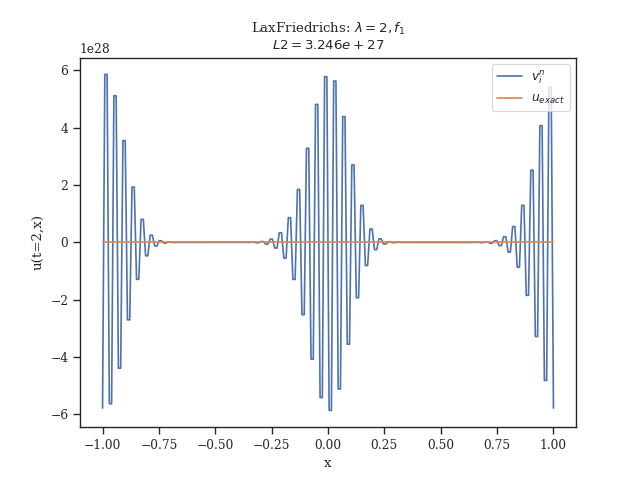
\includegraphics[width=\linewidth]{figures/LaxFriedrichs/LaxFriedrichs_lambda=2,f1}
        \caption{Lax-Friedrichs, $\lambda =2$}
    \end{subfigure}
    \hfill
    \begin{subfigure}{0.3\linewidth}
        \centering
        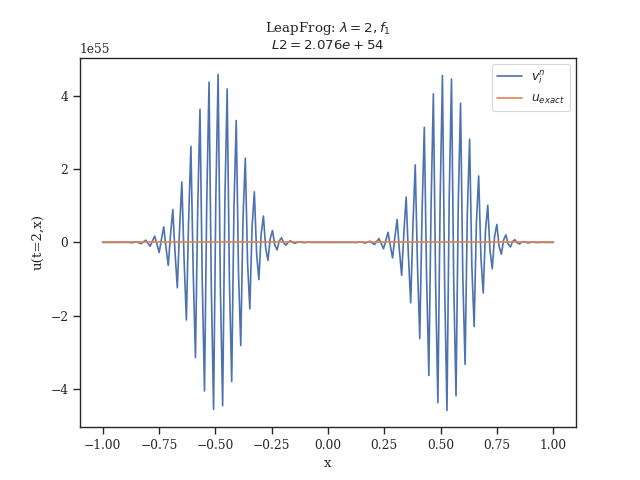
\includegraphics[width=\linewidth]{figures/LeapFrog/LeapFrog_lambda=2,f1}
        \caption{Leap-Frog, $\lambda =2$}
    \end{subfigure}
    \hfill

    \caption{Solutions of Varying $\lambda$ for $f_1$}
    \label{f1 figures}

\end{figure}

\begin{figure}
    \centering
    \begin{subfigure}{0.3\linewidth}
        \centering
        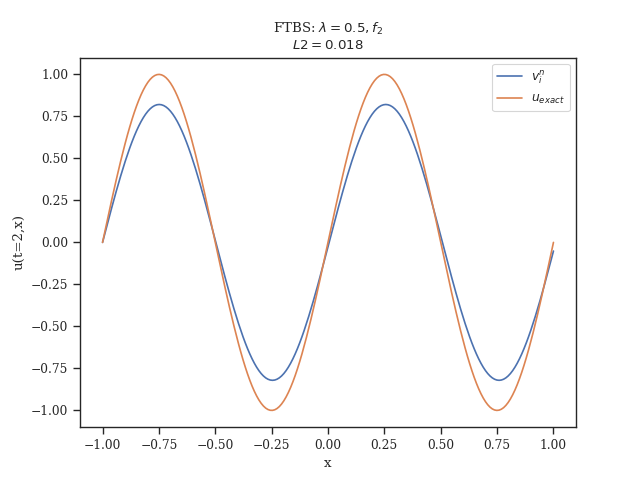
\includegraphics[width=\linewidth]{figures/FTBS/FTBS_lambda=0.5,f2}
        \caption{FTBS, $\lambda = 0.5$}
    \end{subfigure}
    \hfill
    \begin{subfigure}{0.3\linewidth}
        \centering
        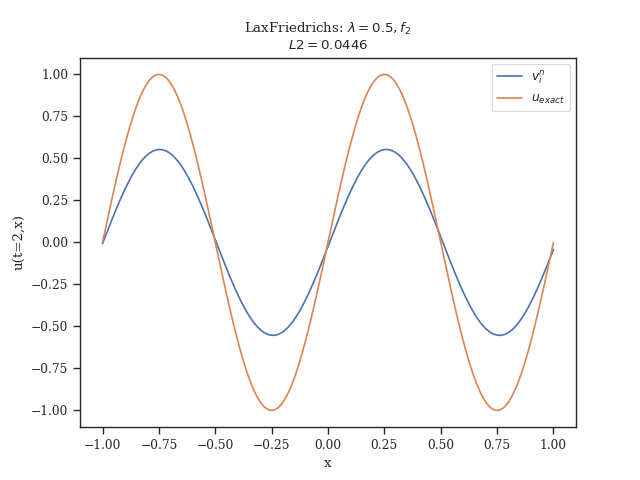
\includegraphics[width=\linewidth]{figures/LaxFriedrichs/LaxFriedrichs_lambda=0.5,f2}
        \caption{Lax-Friedrichs, $\lambda =0.5$}
    \end{subfigure}
    \hfill
    \begin{subfigure}{0.3\linewidth}
        \centering
        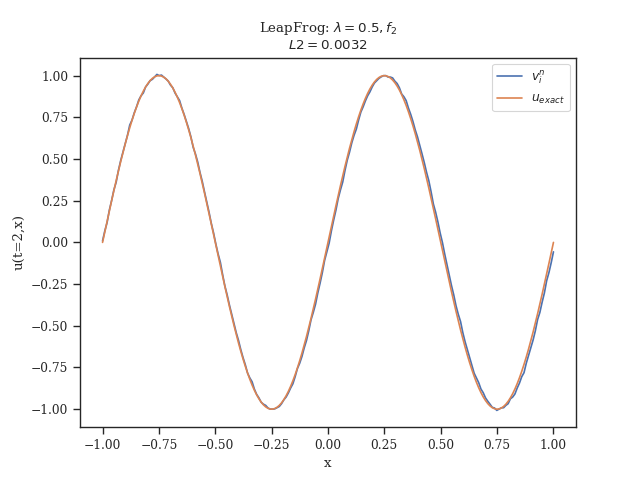
\includegraphics[width=\linewidth]{figures/LeapFrog/LeapFrog_lambda=0.5,f2}
        \caption{Leap-Frog, $\lambda =0.5$}
    \end{subfigure}
    \hfill
    \vspace{1cm}
    \begin{subfigure}{0.3\linewidth}
        \centering
        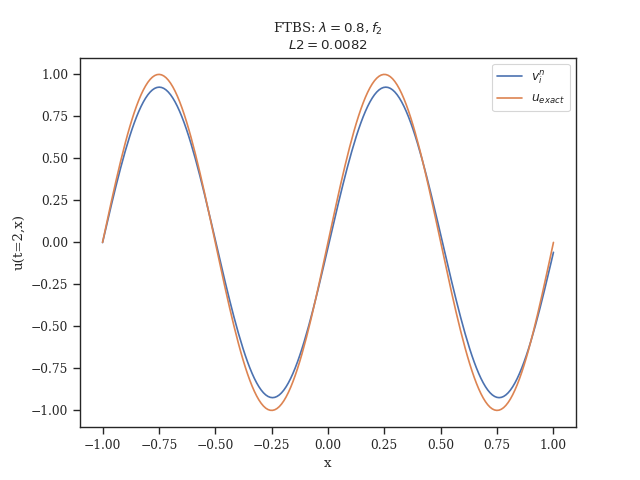
\includegraphics[width=\linewidth]{figures/FTBS/FTBS_lambda=0.8,f2}
        \caption{FTBS, $\lambda = 0.8$}
    \end{subfigure}
    \hfill
    \begin{subfigure}{0.3\linewidth}
        \centering
        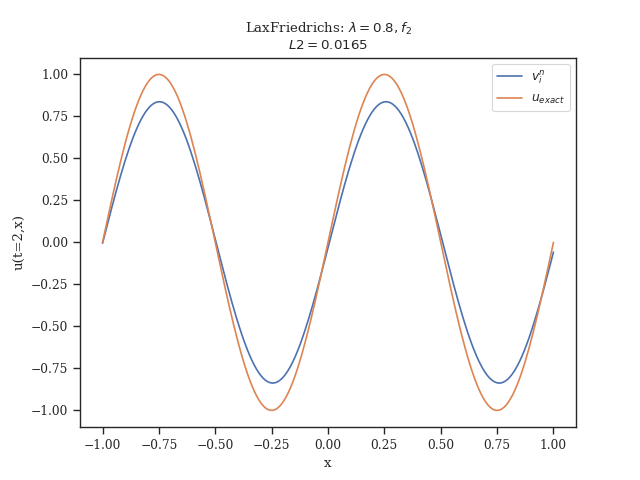
\includegraphics[width=\linewidth]{figures/LaxFriedrichs/LaxFriedrichs_lambda=0.8,f2}
        \caption{Lax-Friedrichs, $\lambda =0.8$}
    \end{subfigure}
    \hfill
    \begin{subfigure}{0.3\linewidth}
        \centering
        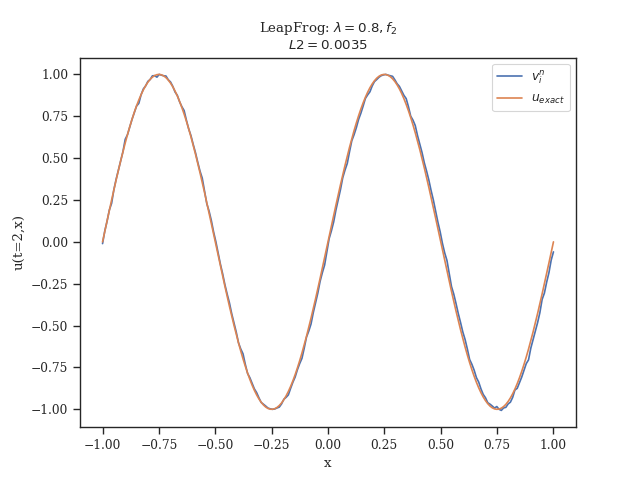
\includegraphics[width=\linewidth]{figures/LeapFrog/LeapFrog_lambda=0.8,f2}
        \caption{Leap-Frog, $\lambda =0.8$}
    \end{subfigure}
    \hfill
    \vspace{1cm}
    \begin{subfigure}{0.3\linewidth}
        \centering
        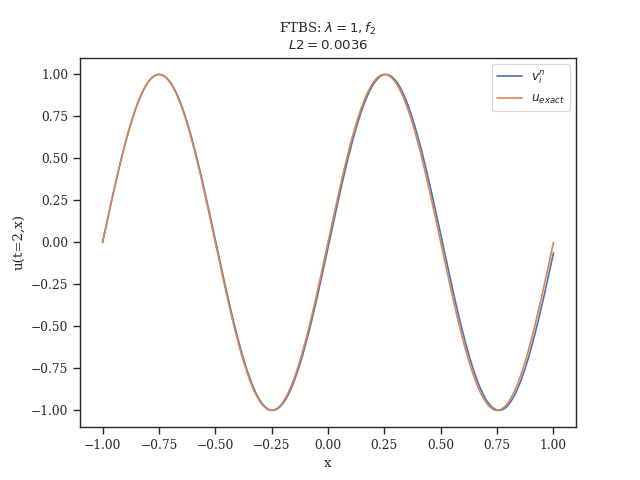
\includegraphics[width=\linewidth]{figures/FTBS/FTBS_lambda=1,f2}
        \caption{FTBS, $\lambda = 1$}
    \end{subfigure}
    \hfill
    \begin{subfigure}{0.3\linewidth}
        \centering
        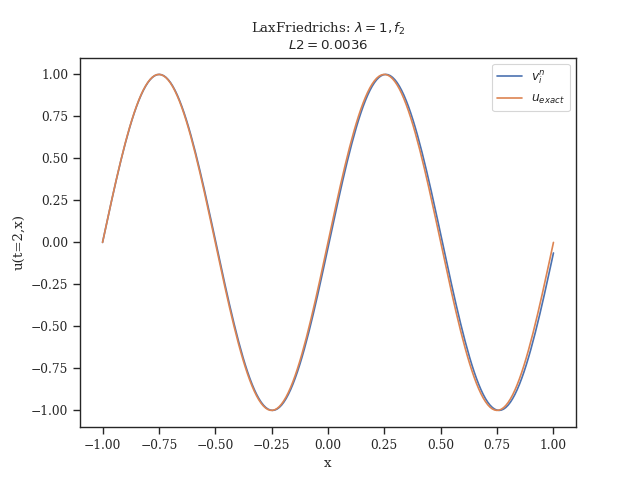
\includegraphics[width=\linewidth]{figures/LaxFriedrichs/LaxFriedrichs_lambda=1,f2}
        \caption{Lax-Friedrichs, $\lambda =1$}
    \end{subfigure}
    \hfill
    \begin{subfigure}{0.3\linewidth}
        \centering
        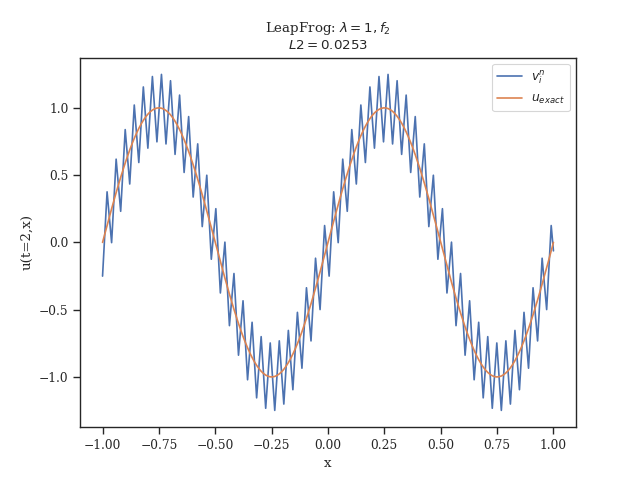
\includegraphics[width=\linewidth]{figures/LeapFrog/LeapFrog_lambda=1,f2}
        \caption{Leap-Frog, $\lambda =1$}
        \label{weird leap frog}
    \end{subfigure}
    \hfill
    \vspace{1cm}
    \begin{subfigure}{0.3\linewidth}
        \centering
        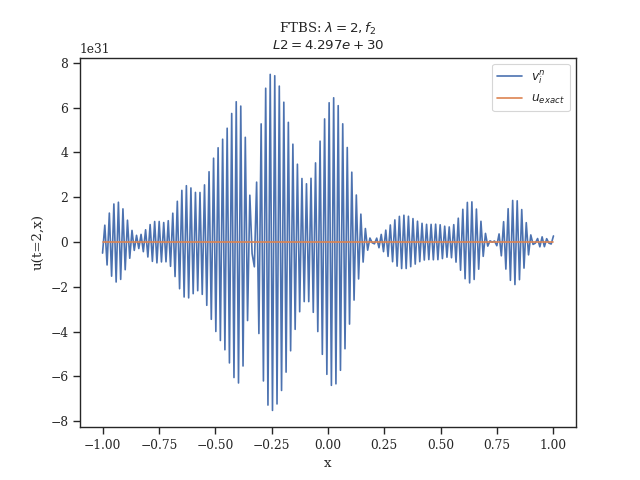
\includegraphics[width=\linewidth]{figures/FTBS/FTBS_lambda=2,f2}
        \caption{FTBS, $\lambda = 2$}
    \end{subfigure}
    \hfill
    \begin{subfigure}{0.3\linewidth}
        \centering
        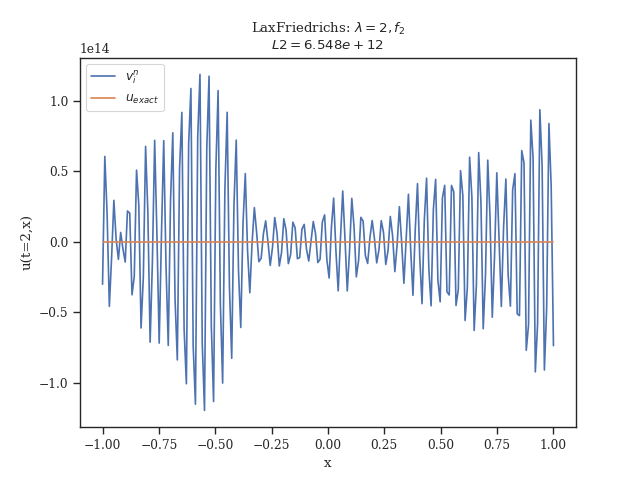
\includegraphics[width=\linewidth]{figures/LaxFriedrichs/LaxFriedrichs_lambda=2,f2}
        \caption{Lax-Friedrichs, $\lambda =2$}
    \end{subfigure}
    \hfill
    \begin{subfigure}{0.3\linewidth}
        \centering
        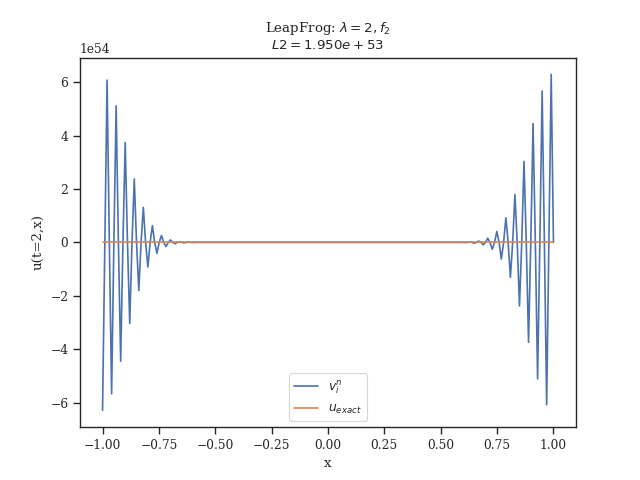
\includegraphics[width=\linewidth]{figures/LeapFrog/LeapFrog_lambda=2,f2}
        \caption{Leap-Frog, $\lambda =2$}
    \end{subfigure}
    \hfill

    \caption{Solutions of Varying $\lambda$ for $f_2$}
    \label{f2 figures}

\end{figure}
\appendix


%    \section{Python Code}
%    \inputminted[linenos, bgcolor=LightGray, fontsize=\footnotesize]{python}{578_HW1.py}